\begin{frame}{Test Site}

	\begin{itemize}
		\itemfill
		\item High Intensity Proton Accelerator (HIPA) at PSI (Cyclotron)
		\item using beam line $\uppi$M1 at Paul Scherrer Institute (PSI)
		\item positive pions ($\uppi^+$) with momentum of \SI{260}{\mega\electronvolt\per c} 
		\item tunable particle fluxes from \orderof{\SI{1}{\kilo\hertz\per cm^2}} to \orderof{\SI{10}{\mega\hertz\per cm^2}}
	\end{itemize}
	
	\begin{figure}
		\centering
		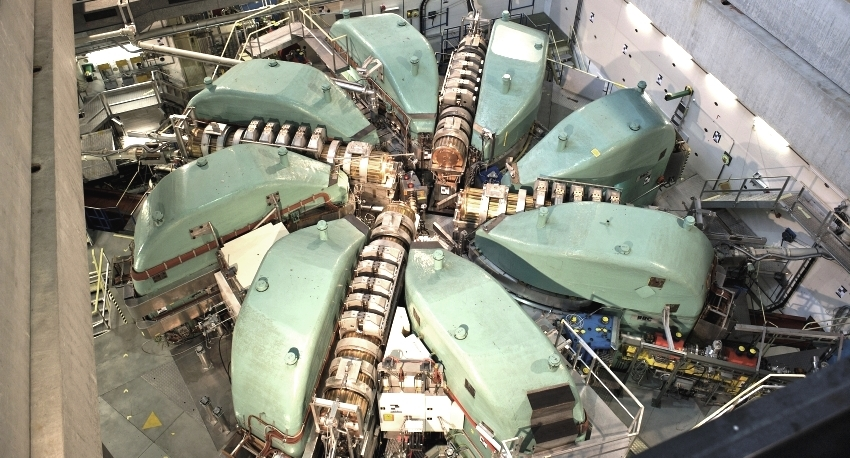
\includegraphics[width=6.5cm]{cyclotron}
	\end{figure}
		
\end{frame}
% ================================ 2 ========================================
\begin{frame}{Setup}
 
	\begin{figure}
		\centering
		\only<1>{
			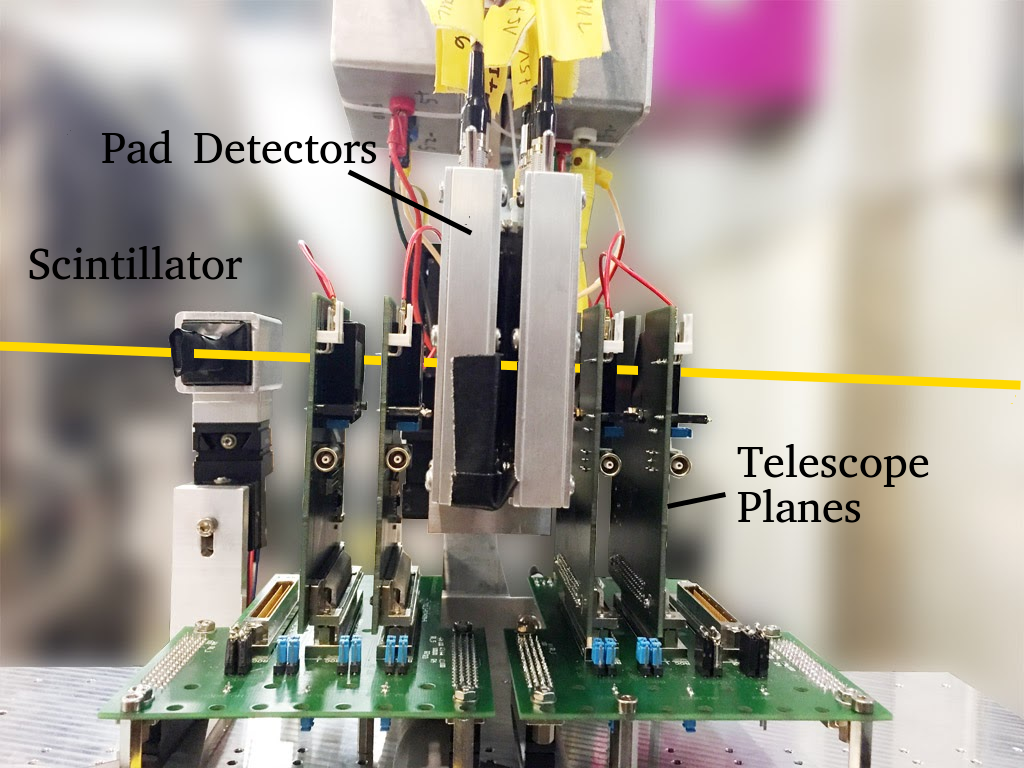
\includegraphics[height=.4\textheight]{Setup}
			\caption{pad telescope}}
		\only<2>{
			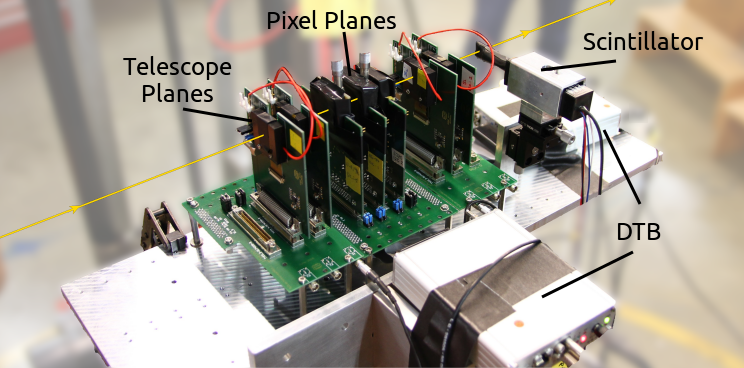
\includegraphics[height=.4\textheight]{PixTel1}
			\caption{pixel telescope}}
	\end{figure}\vspace*{-5pt}
 
	\begin{itemize}
		\itemfill
		\item modular ETH beam telescope \ra test apparatus for all detectors
		\item 4 tracking planes \ra trigger (fast-OR) with scalable area
		\item fast-OR clocked with \SI{40}{\mega\hertz} \ra \SI{25}{\nano\second} time precision
		\item diamond detectors (DUTs) in between tracking planes
		\item scintillator for precise trigger timing \ra \orderof{\SI{1}{\nano\second}}
	\end{itemize}

\end{frame}

% ================================ 3 ========================================
\begin{frame}{Setup}
 
	\begin{figure}
		\centering
		\only<1>{
			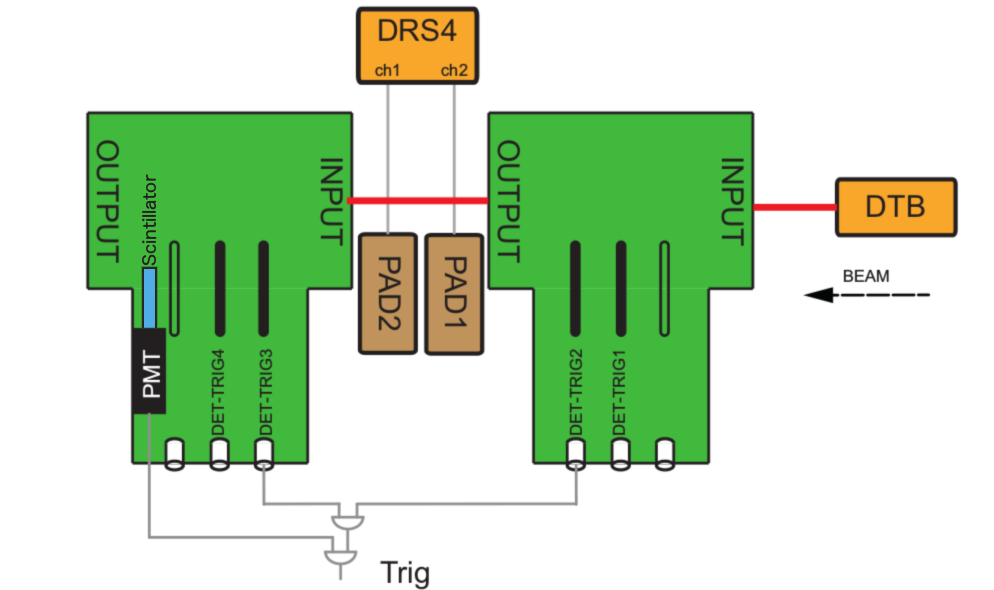
\includegraphics[height=.4\textheight]{SchematicsV2}
			\caption{pad telescope}}
		\only<2>{
			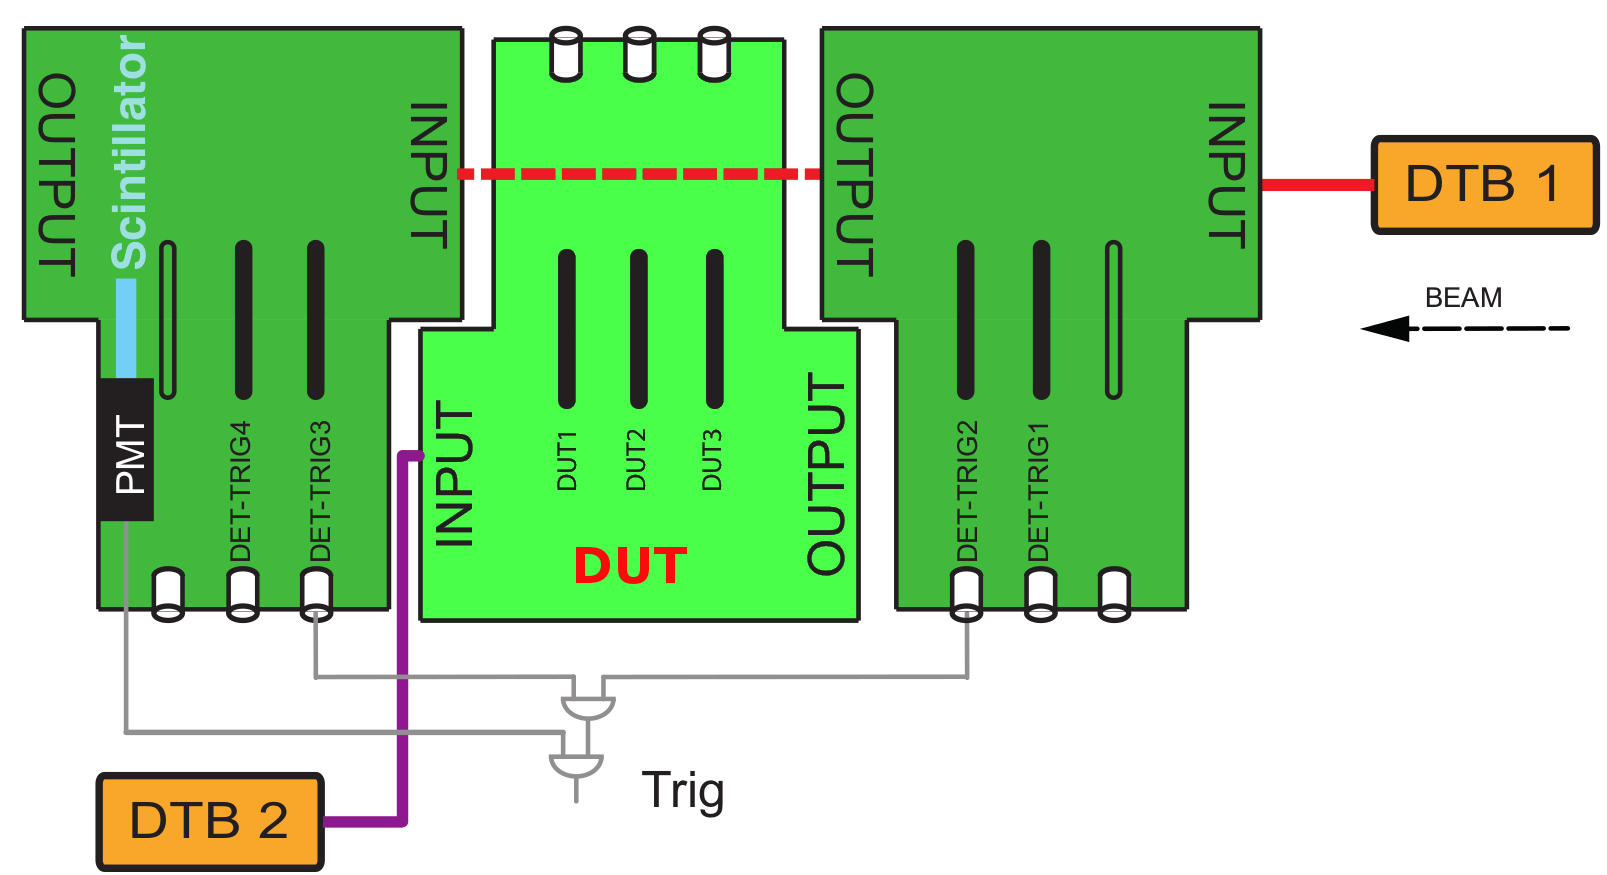
\includegraphics[height=.4\textheight]{TelSchemePix}
			\caption{pixel telescope}}
	\end{figure}\vspace*{-5pt}
 
	\begin{itemize}
		\itemfill
		\only<1>{\item PSI DRS4 Evaluation Board as digitizer for the pad waveforms}
		\only<2>{\item independent telescope module as DUT (light green)}
		\item Digital Test Board (DTB) and pXar software for the telescope readout
		\item global trigger as coincidence of fast-OR self trigger and scintillator signal
		\item EUDAQ as DAQ framework
	\end{itemize}

\end{frame}



